\section{Virtualization}

\begin{definition}[\textit{Machine}]
    A machine serves as an execution environment capable of running programs.
\end{definition}
Computer architecture defines sets of instructions organized into various levels that programs can utilize.
The OS plays a crucial role by creating new instructions and facilitating program access to devices and hardware resources.

\begin{figure}[H]
    \centering
    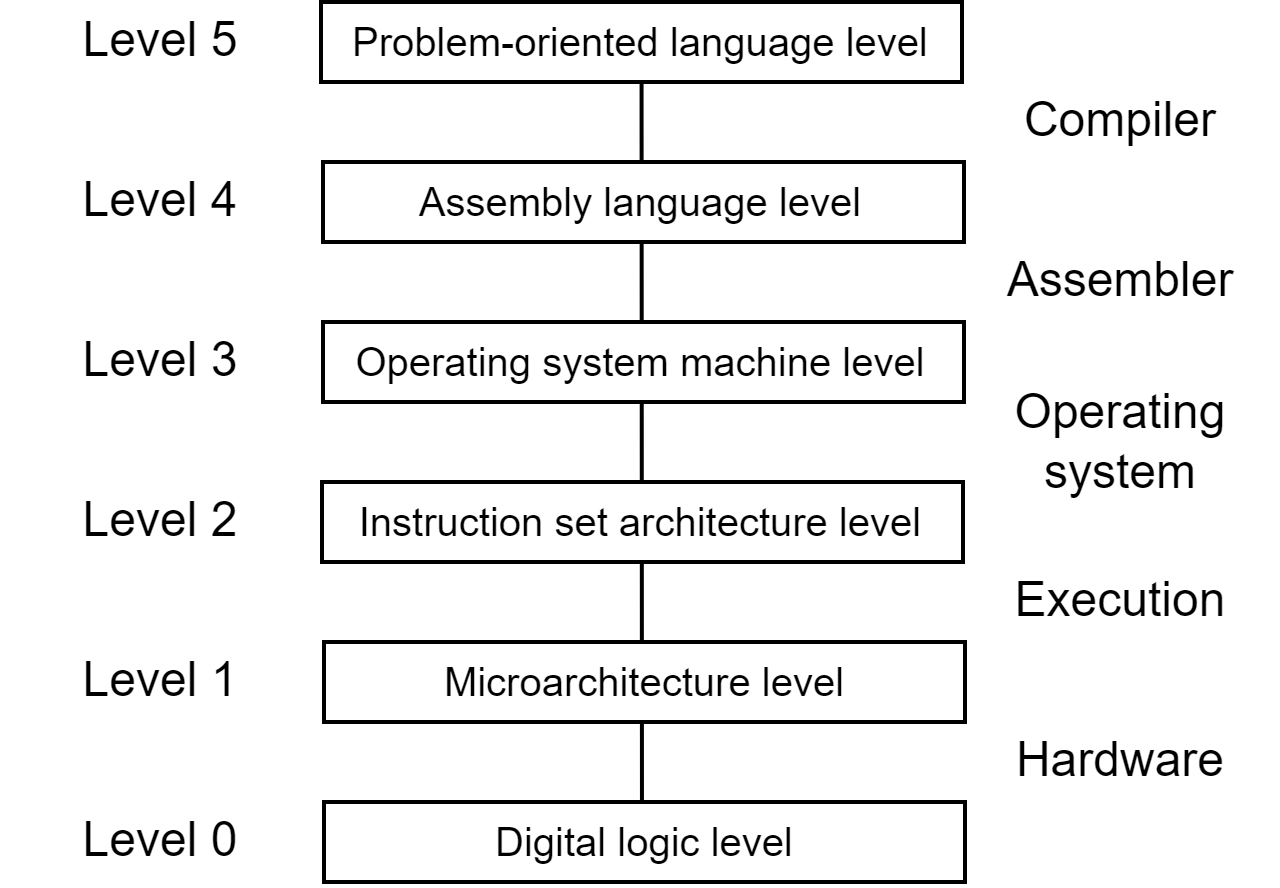
\includegraphics[width=0.5\linewidth]{images/lev.png}
    \caption{Machine's architectures levels}
\end{figure}

The main levels of virtualization include:
\begin{itemize}
    \item \textit{Instruction Set Architecture} (ISA): this is the second level, marking the boundary between hardware and software.
        ISA can be subdivided into:
        \begin{itemize}
            \item \textit{User}: consists of instructions visible to the application program, used for basic arithmetic operations and interfacing directly with the hardware.
            \item \textit{System}: comprises instructions visible to the OS, which manages hardware resources.
                This ISA abstracts CPU complexity, defining how applications access memory and facilitating hardware communication.
        \end{itemize}
    \item \textit{Application Binary Interface} (ABI): this is the third level, serving as the boundary between OS and software.
        The ABI includes aspects of the ISA visible to an application program. 
        System calls are performed indirectly through the OS using shared hardware resources.
        Each machine level executes only its designated instructions, ensuring proper interaction and execution.
\end{itemize}

\subsection{Virtual Machines}
A VM is a logical abstraction providing a virtualized execution environment:
\begin{itemize}
    \item It offers software behavior identical to that of a physical machine.
    \item It consists of both physical hardware and virtualizing software.
    \item It may present different resources than a physical machine.
    \item It may have varying performance levels compared to physical counterparts.
\end{itemize}
The tasks of a VM include mapping virtual resources or states to corresponding physical ones and using physical machine instructions or calls to execute virtual instructions.

There are two primary types of VMs:
\begin{enumerate}
    \item \textit{System VMs}: these emulate an entire physical computer system, including its hardware resources.
        The virtualizing software is positioned at the ISA interface.
        System VMs offer a complete system environment capable of supporting an OS and multiple user processes, granting the OS access to underlying hardware resources.
        The virtualization software, commonly called VMM, operates directly on the hardware or on top of another OS.
    \item \textit{Process VMs}: these provide a virtualized environment for individual processes.
        The virtualizing software is positioned at the ABI interface and is referred to as Runtime Software.
        Runtime software supporting process VMs typically spans three levels of the architecture.
\end{enumerate}
\begin{definition}[\textit{Host}]
    The host is the underlying platform that supports the virtualized environment.
\end{definition}
\begin{definition}[\textit{Guest}]
    The guest is the software that operates within the VM environment.
\end{definition}
\begin{figure}[H]
    \centering
    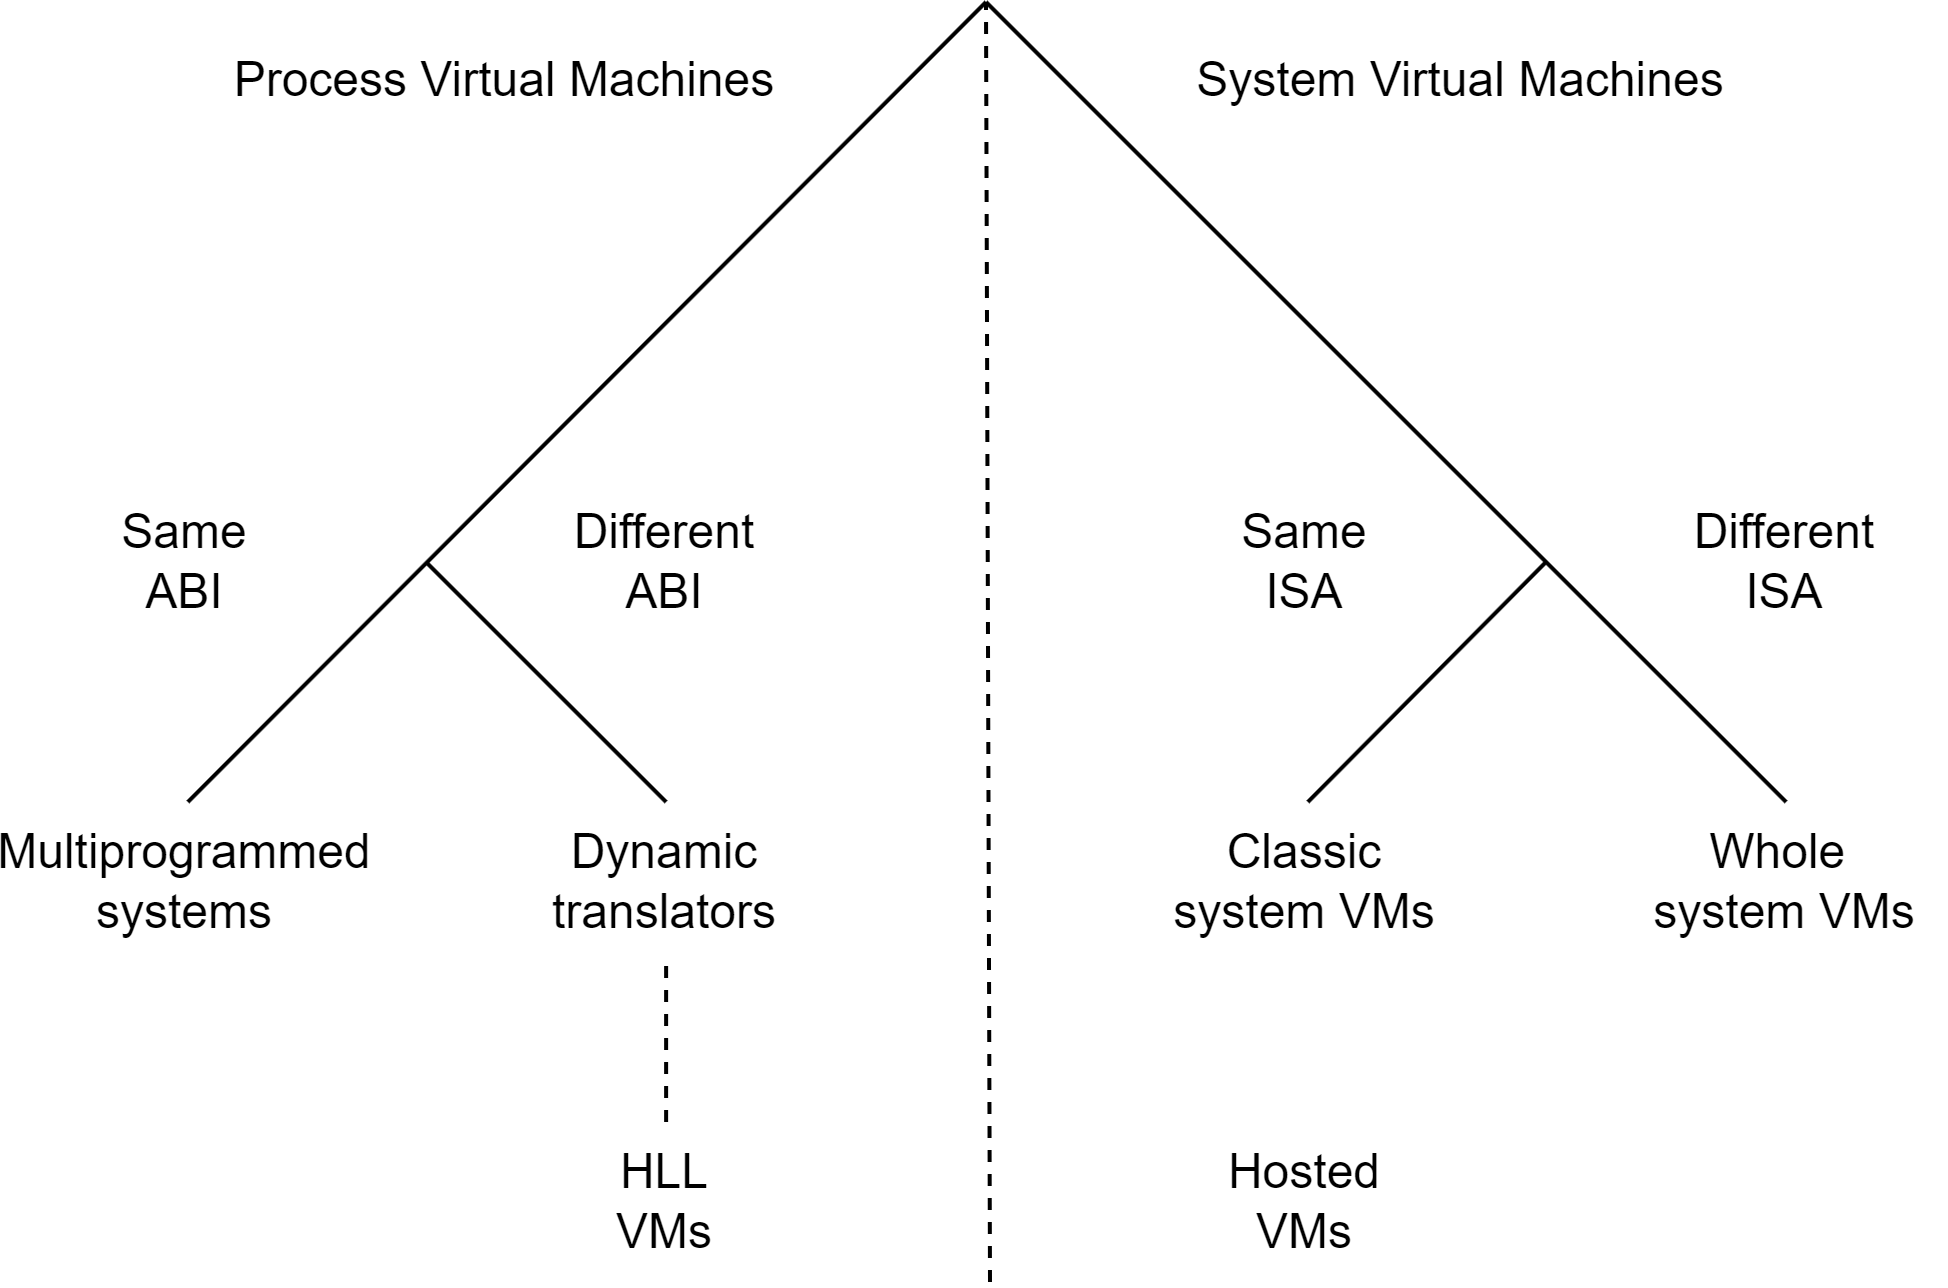
\includegraphics[width=0.5\linewidth]{images/vtyp.png}
    \caption{Virtual Machines taxonomy}
\end{figure}

\paragraph*{System VMs}
System VMs can use the same or different ISA. 
Based on this, we have:
\begin{itemize}
    \item \textit{Classic systems} (same ISA): the VMM resides directly on the hardware, managing interactions between the guest OS and hardware resources.
        This configuration efficiently supports the execution of different OS on the same hardware platform.
    \item \textit{Whole system} (different ISA): the VMM resides on top of an existing OS, with all software components virtualized.
        Due to the different ISAs, both application and OS code require emulation via binary translation.
\end{itemize}

\paragraph*{Process VMs}
Process VMs can use the same or different ABI. 
Based on this, we have:
\begin{itemize}
    \item \textit{Multi-programmed systems} (same ABI): VMs are formed by the OS call interface and the user ISA.
        This approach supports multiple users by giving each process the illusion of having exclusive access to a complete machine, with the OS managing resource distribution.
    \item \textit{High-level language system} (different ABI): provide isolated execution environments for applications or multiple instances.
        They translate application bytecode into OS-specific executable code while minimizing dependencies on hardware and OS.
        Applications run normally but with characteristics like isolation and multi-environment support, without adhering to traditional installation processes.
\end{itemize}

\paragraph*{Emulation}
Emulation involves developing software technologies that enable an application or OS to operate in an environment different from its original platform.
An emulator reads all bytes in the system memory it seeks to replicate.
A common emulation method is interpretation, where an interpreter program sequentially fetches, decodes, and emulates the execution of individual source instructions. 
This method, though often slow, allows for the replication of different platform environments.

\subsection{Implementation levels}
In implementing virtualization within a typical layered system architecture, additional layers are introduced between existing layers. 
Depending on their placement, various types of virtualization can be achieved:
\begin{itemize}
    \item \textit{Hardware-level virtualization}: the virtualization layer is situated between the hardware and the OS.
        This configuration alters the interface seen by the OS and applications, which might differ from the physical hardware interface.
    \item \textit{Application-level virtualization}: this layer is placed between the OS and specific applications.
        It ensures that applications receive a consistent interface, allowing them to run within their own environment independently of the OS.
    \item \textit{System-level virtualization}: the virtualization layer provides the interface of a physical machine to a secondary OS and the applications running within it.
        This layer is positioned between the system's primary OS and other OS instances, enabling multiple OS to run on a single hardware infrastructure.
\end{itemize}

\subsection{Virtual Machines properties}
VMs possess several key properties:
\begin{itemize}
    \item \textit{Partitioning}: multiple OS can run on a single physical machine with partitioned resources.
    \item \textit{Isolation}: ensuring that each VM operates independently and securely.
    \item \textit{Advanced resource control}: efficient and flexible management of resources.
    \item \textit{Encapsulation}: the state of a VM can be saved in a file, simplifying replication and migration processes.
    \item \textit{Hardware independence}: VMs can run on various hardware platforms without modification.
\end{itemize}

\subsection{Virtual Machines Managers}
A Virtual Machine Manager (VMM), also known as a Hypervisor, is responsible for mediating access to hardware resources on the physical host system.
It intercepts and handles any privileged or protected instructions issued by the VMs.
Typically, a VMM runs VMs with OS, libraries, and utilities compiled for the same type of processor and instruction set as the physical machine.

\begin{figure}[H]
    \centering
    \begin{subfigure}{0.4\textwidth}
        \centering
        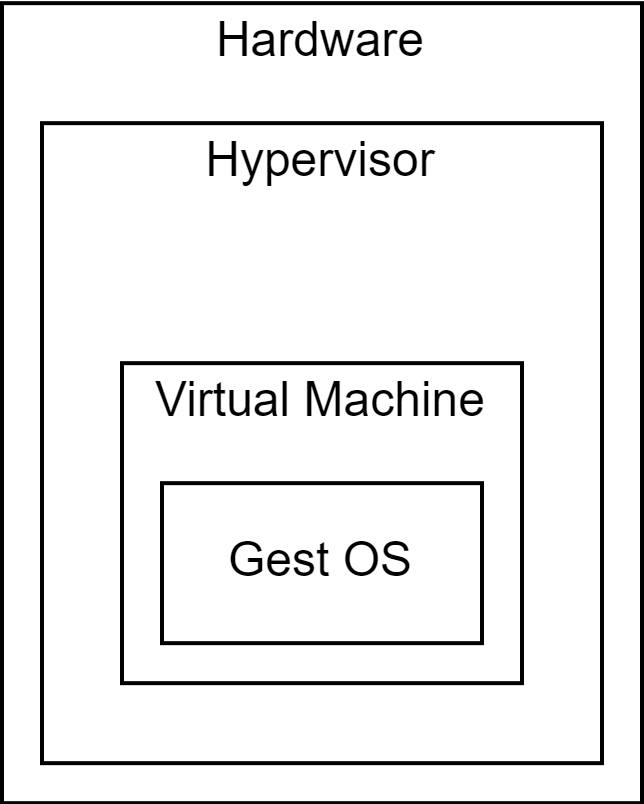
\includegraphics[width=0.75\linewidth]{images/hyp1.png} 
        \caption{Hypervisor type one}
    \end{subfigure}
    \begin{subfigure}{0.4\textwidth}
        \centering
        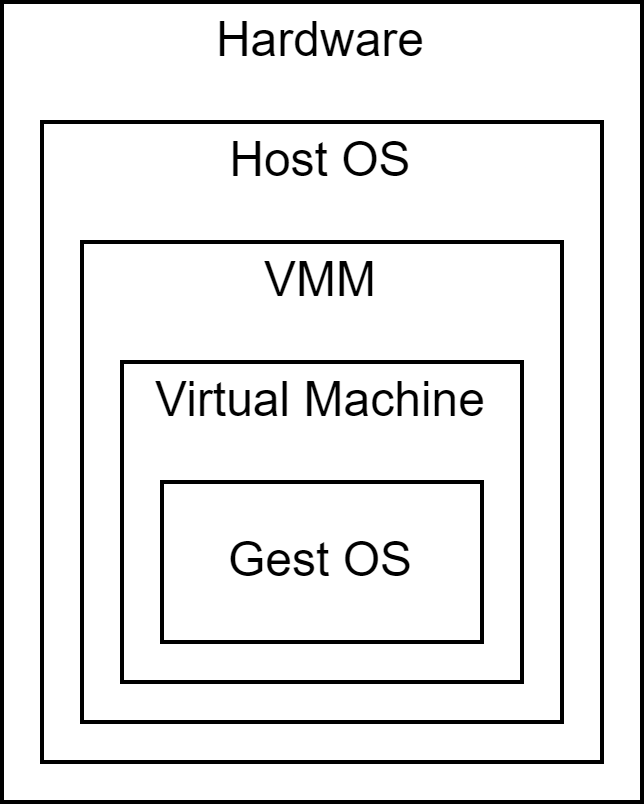
\includegraphics[width=0.75\linewidth]{images/hyp2.png}
        \caption{Hypervisor type two}
    \end{subfigure}
    \caption{Hypervisor types}
\end{figure}

Hypervisors are classified into two types:
\begin{itemize}
    \item \textit{Type one} (bare metal): directly controls the hardware without requiring an underlying OS.
        The architecture can be: 
        \begin{itemize}
            \item \textit{Monolithic}: device drivers run within the Hypervisor itself, offering better performance and isolation but limited to hardware supported by the Hypervisor.
            \item \textit{Microkernel}: device drivers run within a service VM, resulting in a smaller Hypervisor. 
                This approach leverages the driver ecosystem of an existing OS and allows the use of third-party drivers.
        \end{itemize}

        \begin{figure}[H]
            \centering
            \begin{subfigure}{0.4\textwidth}
                \centering
                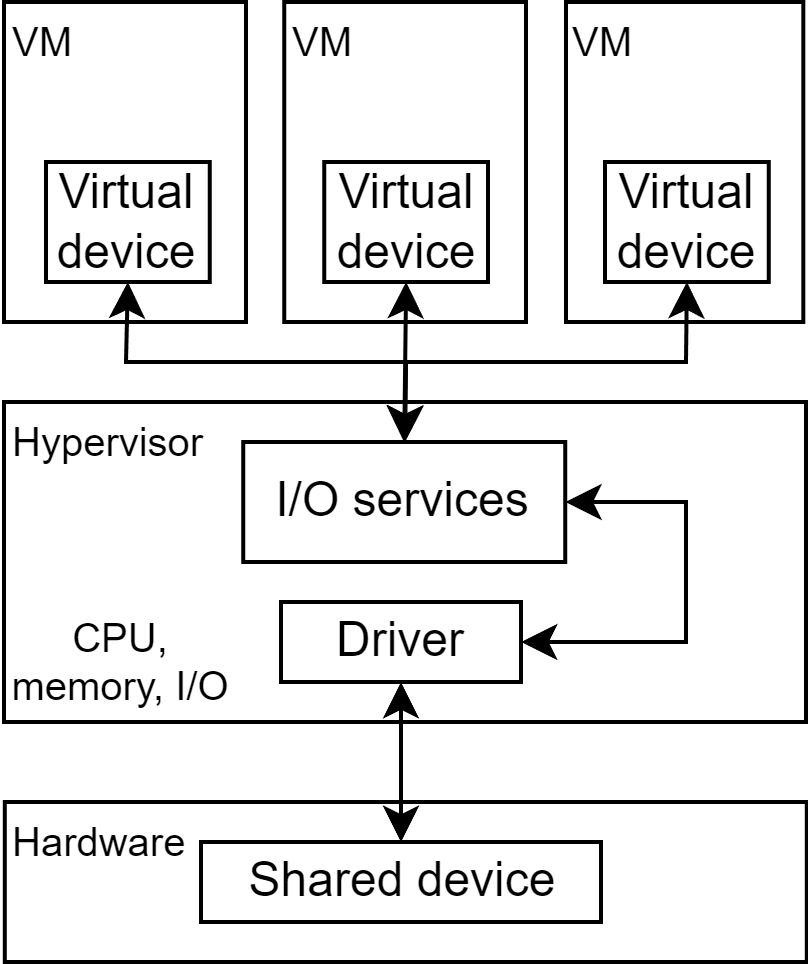
\includegraphics[width=0.75\linewidth]{images/mono.png} 
                \caption{Monolithic}
            \end{subfigure}
            \begin{subfigure}{0.4\textwidth}
                \centering
                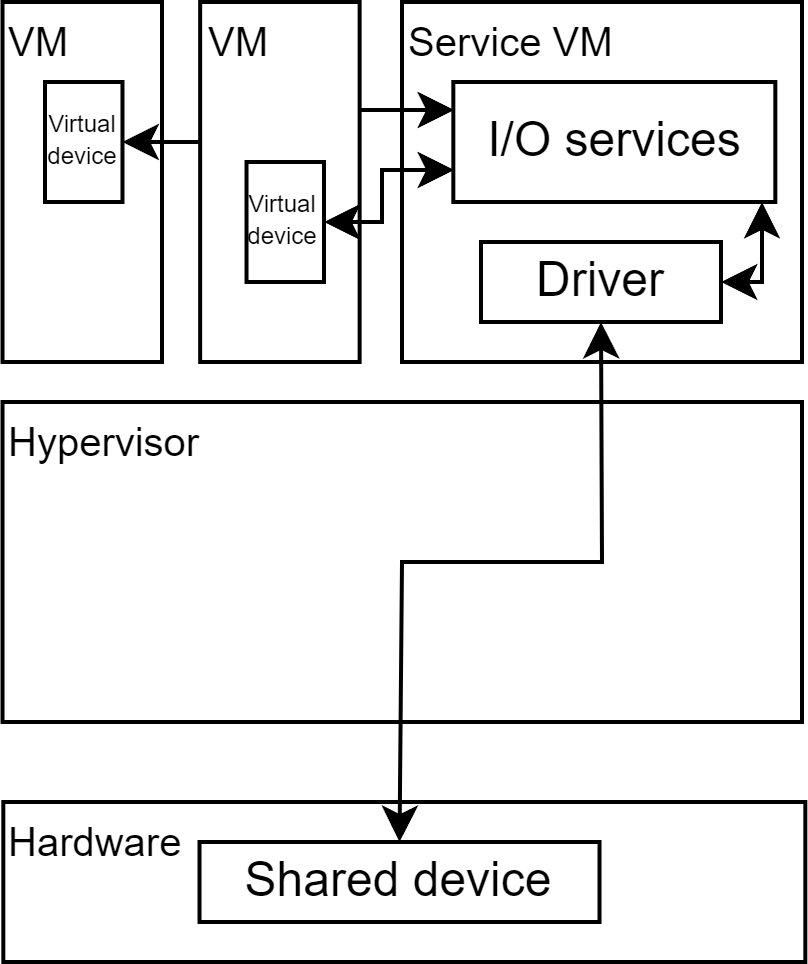
\includegraphics[width=0.75\linewidth]{images/mic.png}
                \caption{Microkernel}
            \end{subfigure}
            \caption{Type one Hypervisor architectures}
        \end{figure}

    \item \textit{Type two} (VMM): requires a host OS for CPU scheduling and memory management. 
        The host OS runs the VM, and the guest OS runs within the VM.
        This type is easily configurable but needs caution to prevent conflicts between the host OS and guest OS.
\end{itemize}

\subsection{System level virtualization techniques}
There are various methods to implement system level virtualization:
\begin{itemize}
    \item \textit{Paravirtualization}: involves collaboration between the guest OS and the VM.
        The VMM provides a virtual interface that resembles the underlying hardware, aiming to reduce resource-intensive tasks in the virtualized environment.
        This approach simplifies VMM implementation and enhances performance but requires modifications to the guest OS and is incompatible with traditional OSs.
    \item \textit{Full virtualization}: provides a complete simulation of the underlying hardware.
        The Hypervisor intercepts and manages protected instructions, allowing unmodified OSs to run. 
        However, this approach relies on Hypervisor mediation for communication between guests and hosts and requires specific hardware support.
\end{itemize}

\begin{figure}[H]
    \centering
    \begin{subfigure}{0.49\textwidth}
        \centering
        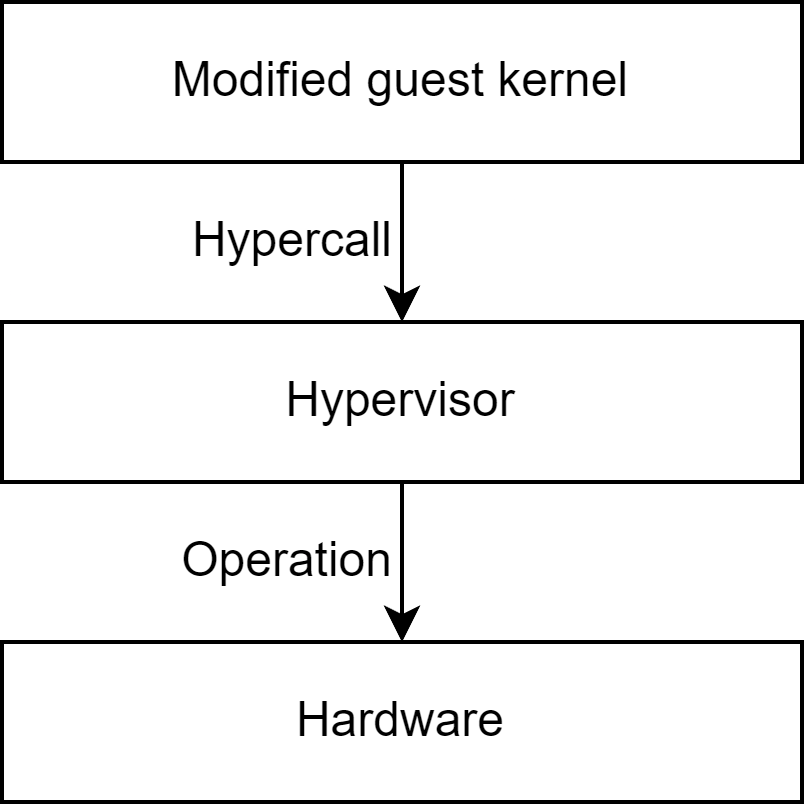
\includegraphics[width=0.75\linewidth]{images/para.png} 
        \caption{Paravirtualization}
    \end{subfigure}
    \begin{subfigure}{0.49\textwidth}
        \centering
        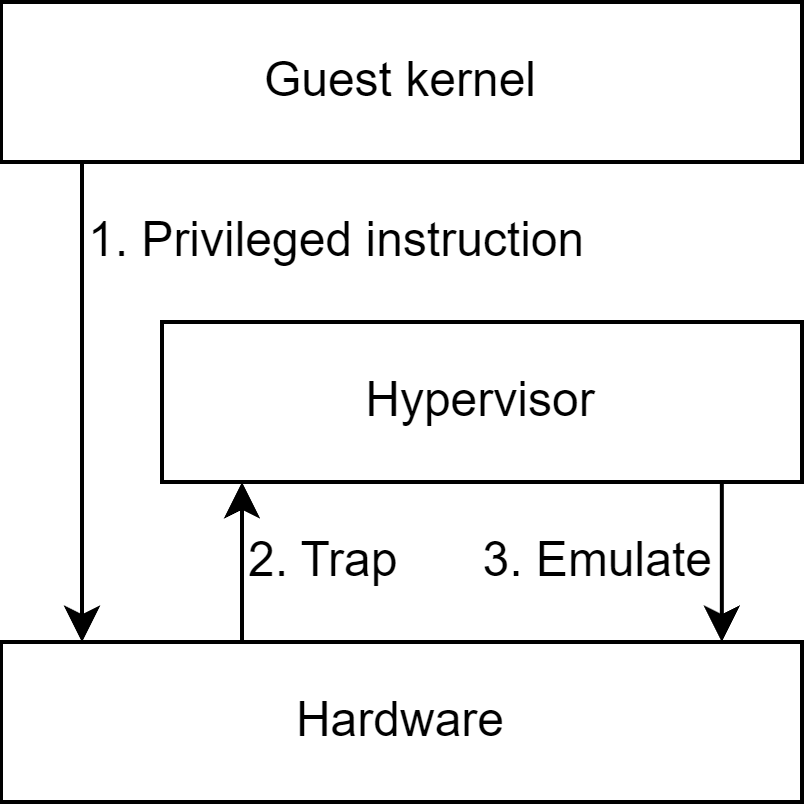
\includegraphics[width=0.75\linewidth]{images/full.png}
        \caption{Full virtualization}
    \end{subfigure}
    \caption{System level virtualization techniques}
\end{figure}